\section{From pupil field to image field}
\subsection{A pupil map is not an image}
Let $A(x_p,y_p)$ be the real nonnegative pupil amplitude and $W(x_p,y_p)$ the residual optical path difference from an ideal converging reference wave. For an image point a distance $f$ away, the paraxial exit-pupil field is
\begin{equation}
U_p(x_p,y_p)=A(x_p,y_p)
\exp\!\left[-\frac{\ii k_0}{2f}(x_p^2+y_p^2)\right]
\exp[\ii k_0W(x_p,y_p)].
\end{equation}
The quadratic phase is the ideal convergence. The residual $W$ measures departures from that reference, not the physical height of a wafer surface.

Fresnel propagation to the reference image plane gives
\begin{align}
U_f(\xi,\eta)&=\frac{\ee^{\ii k_0f}}{\ii\lambda_0 f}
\iint U_p(x_p,y_p)
\exp\!\left[\frac{\ii k_0}{2f}\big((\xi-x_p)^2+(\eta-y_p)^2\big)\right]
\dd x_p\dd y_p.\nonumber
\end{align}
Expand the squares. The pupil-quadratic terms cancel; the remaining image-quadratic phase has unit magnitude and does not affect intensity:
\begin{equation}
\boxed{U_f(\xi,\eta)=C(\xi,\eta)
\iint A\ee^{\ii k_0W}
\ee^{-\ii k_0(x_p\xi+y_p\eta)/f}\dd x_p\dd y_p,}
\label{eq:fourier}
\end{equation}
where $C=\ee^{\ii k_0f}\ee^{\ii k_0(\xi^2+\eta^2)/(2f)}/(\ii\lambda_0 f)$.
With $(x_p,y_p)=a(u,v)$ and $s_x=\NA\xi/\lambda_0$, $s_y=\NA\eta/\lambda_0$, $\NA\simeq a/f$ in vacuum,
\begin{equation}
U_f\propto\int_{u^2+v^2\leq1}A(u,v)\ee^{\ii2\pi W/\lambda_0}
\ee^{-\ii2\pi(us_x+vs_y)}\dd u\dd v,\qquad
I_f\propto|U_f|^2.
\label{eq:fft}
\end{equation}
% \point{The map displays a phase error indexed by pupil position. The image is the interference of contributions from the \emph{whole} pupil. A red lobe in a pupil map is not a red or bright lobe at the same position in the image.}

For $W=0$ and $A=1$ on a disk, angular integration gives
$\int_0^{2\pi}\ee^{-\ii2\pi s\rho\cos\theta}\dd\theta=2\pi J_0(2\pi s\rho)$, and the radial integral gives the normalized amplitude
\begin{equation}
\frac{U_f(s)}{U_f(0)}=\frac{2J_1(2\pi s)}{2\pi s},\qquad
I_f(s)/I_f(0)=\left[\frac{2J_1(2\pi s)}{2\pi s}\right]^2.
\end{equation}
Its first dark ring is at $s\simeq0.610$, or image radius $0.610\lambda_0/\NA$.

\subsection{Wavefront slopes give ray displacements}
The local phase and its gradients are
\begin{align}
\Phi(x_p,y_p)&=-\frac{k_0}{2f}(x_p^2+y_p^2)+k_0W(x_p,y_p),\\
\frac{k_x}{k_0}&=-\frac{x_p}{f}+\frac{\partial W}{\partial x_p},&
\frac{k_y}{k_0}&=-\frac{y_p}{f}+\frac{\partial W}{\partial y_p}.
\end{align}
For small ray angles, propagation over $f$ produces
\begin{equation}
\xi\simeq x_p+f\frac{k_x}{k_0}
=x_p-x_p+f\frac{\partial W}{\partial x_p},
\end{equation}
and similarly for $\eta$. Therefore
\begin{equation}
\boxed{(\xi,\eta)=f\nabla_pW
=\frac{f}{a}\left(\frac{\partial W}{\partial u},\frac{\partial W}{\partial v}\right).}
\label{eq:rays}
\end{equation}
The same result follows by stationary phase in \eqref{eq:fourier}:
$\partial_{x_p}(W-x_p\xi/f-y_p\eta/f)=0$.
Thus the ray relation and diffraction integral agree under the same sign convention. Rays describe local phase directions; diffraction determines the finite intensity distribution, including interference and the Airy scale.

% \note{In a lossless image medium of index $n_i$, retain phase error $k_0W$, but replace the ideal propagation wave number by $n_i k_0$. Then $(\xi,\eta)=(f/(n_i a))\nabla_{u,v}W$, and $\NA\simeq n_i a/f$. The vacuum formulas are adequate for this teaching model.}

\subsection{Piston and tilt: two exact field results}
For piston $W=p$, \eqref{eq:fourier} simply acquires $\ee^{\ii k_0p}$, so intensity is unchanged everywhere. Likewise \eqref{eq:rays} gives zero ray displacement. Global piston cannot be recovered from an intensity-only image of this isolated field; an external coherent reference would change the measurement.

For tilt $W=t_xu+t_yv$, combine the linear phases in \eqref{eq:fft}:
\begin{equation}
\boxed{I_f(\xi,\eta)=I_0\!\left(\xi-\frac{f}{a}t_x,
\eta-\frac{f}{a}t_y\right),\qquad
\Delta\mathbf x=\frac{f}{a}(t_x,t_y).}
\label{eq:tiltphysical}
\end{equation}
An irrelevant unit-modulus image phase may differ between the corresponding complex fields. All pupil rays receive the same displacement. Shape is unchanged, while placement is changed. Recentring an image removes this placement information; a tilt-removed RMS cannot bound the removed shift.

\textbf{Reconciliation with textbook \S6.4.} That section uses a \emph{spatial-frequency pupil} with the inverse Fourier kernel $\ee^{+\ii2\pi\boldsymbol\nu\cdot\mathbf x}$. It consequently writes $\Delta\mathbf x=-\mathbf t_{\rm freq}/\NA$. Equation \eqref{eq:fourier} uses the physical pupil with the negative kernel. Identifying $\boldsymbol\nu=-(x_p,y_p)/(\lambda_0 f)$ reverses the normalized pupil axes, so $\mathbf t_{\rm freq}=-\mathbf t$. The physical predictions agree. The HTML and plots use the positive displacement in \eqref{eq:tiltphysical}.

\subsection{Defocus: change the observation plane}
At $z=f+\Delta z$, expand $1/z\simeq1/f-\Delta z/f^2$. After combining propagation and ideal lens phases, the added residual OPD is
\begin{equation}
W_{\rm focus}=-\frac{\Delta z}{2f^2}(x_p^2+y_p^2)
=-\frac{a^2\Delta z}{2f^2}\rho^2.
\label{eq:focus}
\end{equation}
Equivalently, combining $W=d\rho^2$ with the ideal focusing phase gives $1/f_{\rm new}=1/f-2d/a^2$. At leading order, this pupil error is compensated by
\begin{equation}
\Delta z=\frac{2f^2d}{a^2},\qquad
(\xi,\eta)_{z=f}=\frac{2fd}{a}(u,v).
\end{equation}
The ray spot at the original plane is a disk for a uniformly filled pupil. A common change of focus can remove defocus; it cannot remove all higher-order shapes. Best-focus and fixed-plane results therefore answer different questions.

\section{Deriving the five third-order aberration families}
\subsection{Why these terms occur}
For a centred, rotationally symmetric system let the normalized field vector be $\mathbf h$ and pupil vector $\mathbf u=(u,v)$. Reflection-symmetric scalar polynomials can be built from $\mathbf u^2$, $\mathbf h^2$, and $\mathbf h\cdot\mathbf u$. Once the paraxial reference is chosen, the lowest classical residual wave terms have total degree four. The independent pupil-dependent terms are
$(\mathbf u^2)^2$, $\mathbf u^2(\mathbf h\cdot\mathbf u)$,
$(\mathbf h\cdot\mathbf u)^2$, $\mathbf h^2\mathbf u^2$, and
$\mathbf h^2(\mathbf h\cdot\mathbf u)$. A pure $\mathbf h^4$ term is pupil-constant piston.

Choose the field along $x$, $\mathbf h=(h,0)$, and set $\rho^2=u^2+v^2$:
\begin{equation}
\boxed{W=A\rho^4+Bh\,u\rho^2+Ch^2u^2+Dh^2\rho^2+Eh^3u.}
\label{eq:seidel}
\end{equation}
Here $A,\ldots,E$ have length units; numerical factors are absorbed into their definitions. These are the classical Seidel families. They are fourth degree in the wave expansion but give \emph{third-order ray errors} after a pupil derivative. \textbf{These five forms are consequences of geometrical symmetry, not a universal list of all possible wavefront errors.} Centring, axial rotational symmetry, and reflection symmetry restrict the allowed invariants. Off-axis geometries, decentring, tilt/misalignment, non-axisymmetric surfaces, or other broken symmetries can allow additional terms and different field dependencies. The scalar Fourier integral and wavefront-gradient relation do not require that five-term classification; their own paraxial/scalar assumptions still apply.

\subsection{Spherical aberration: a pupil-radius-dependent focus}
For $W=A(u^2+v^2)^2$, differentiate explicitly:
\begin{equation}
\frac{\partial W}{\partial u}=4Au(u^2+v^2),\qquad
\frac{\partial W}{\partial v}=4Av(u^2+v^2).
\end{equation}
Equation \eqref{eq:rays} gives
\begin{equation}
(\xi,\eta)=\frac{4fA}{a}\rho^2(u,v),\qquad
r_{\rm spot}=\frac{4f|A|}{a}\rho^3.
\end{equation}
The ideal reference sphere has already been subtracted; the quartic here is residual error, not the ideal sphere itself. All rays on a pupil annulus have the same radial displacement; marginal rays deviate most. The radial direction after the pupil is
$\theta_r\simeq-a\rho/f+4A\rho^3/a$. Its axial intercept is
\begin{equation}
z_{\rm axis}\simeq\frac{f}{1-4fA\rho^2/a^2}
\simeq f+\frac{4f^2A}{a^2}\rho^2.
\end{equation}
The focal position depends on pupil radius. One defocus adjustment changes all radii together and cannot make this quartic term vanish. Adding defocus to minimize RMS produces balanced spherical aberration, derived below in the Zernike section.

\subsection{Coma: displaced annular ray circles}
Write $b=Bh$. Then $W=bu(u^2+v^2)=b(u^3+uv^2)$, hence
\begin{equation}
\boxed{(\xi,\eta)=\frac{fb}{a}(3u^2+v^2,\,2uv).}
\end{equation}
On a fixed pupil annulus $u=\rho\cos\theta$, $v=\rho\sin\theta$,
\begin{equation}
(\xi,\eta)=\frac{fb\rho^2}{a}(2+\cos2\theta,\,\sin2\theta).
\end{equation}
Opposite pupil points $(u,v)$ and $(-u,-v)$ have identical coma displacement because both derivatives are even under this inversion. Unlike tilt, however, the displacement varies over the pupil, so recentering cannot remove its blur. Each annulus maps to a circle of radius $|fb|\rho^2/a$ centred at
$(2fb\rho^2/a,0)$. Both radius and offset grow with $\rho^2$, producing the asymmetric family of intercepts associated with coma. Diffraction turns this geometrical tendency into a lopsided point image; it is not obtained by colouring these circles as a pupil map.

Balanced Zernike coma subtracts a tilt component from this monomial. That balances its pupil inner product with tilt; it does \emph{not} guarantee that every ray-centroid or peak-position definition vanishes.

\subsection{Astigmatism: two directional foci}
Take $W=c u^2$ with $c=Ch^2$. At the nominal plane,
\begin{equation}
(\xi,\eta)=\frac{2fc}{a}(u,0).
\end{equation}
The pupil collapses geometrically to a line in this particular reference plane. To see the two foci, retain the accompanying isotropic term $d\rho^2$, $d=Dh^2$:
\begin{equation}
W=(c+d)u^2+dv^2,
\qquad
\begin{cases}
\Delta z_x=2f^2(c+d)/a^2,\\
\Delta z_y=2f^2d/a^2.
\end{cases}
\end{equation}
At $\Delta z_x$, the $x$ dependence is focused and the remaining ray line lies along $y$; at $\Delta z_y$, the line lies along $x$. At their midpoint, the effective pupil error is
\begin{equation}
W_{\rm mid}=\frac c2(u^2-v^2)=\frac c2\rho^2\cos2\theta,
\qquad (\xi,\eta)=\frac{fc}{a}(u,-v).
\end{equation}
The ray footprint there is circular for a circular pupil, even though the wavefront is astigmatic. This is a particularly useful warning against reading image shape directly from the pupil map. The two directional focal planes still differ.

\subsection{Field curvature: best focus depends on field position}
For $W=Dh^2\rho^2$,
\begin{equation}
(\xi,\eta)=\frac{2fDh^2}{a}(u,v),\qquad
\Delta z_{\rm best}(h)=\frac{2f^2Dh^2}{a^2}.
\end{equation}
At any one field point this is simply defocus. Its distinguishing feature is the $h^2$ dependence across the field. A curved focal surface can have locally sharp images while a flat wafer is out of focus away from the centre.

The raw astigmatic term contains an isotropic part:
\begin{equation}
Ch^2u^2=\frac{Ch^2}{2}\rho^2\cos2\theta+\frac{Ch^2}{2}\rho^2.
\end{equation}
Consequently the mean focal surface in \eqref{eq:seidel} depends on $(D+C/2)h^2$. Separating field curvature from astigmatism must respect the chosen coefficient convention.

\subsection{Distortion: field-dependent placement without local blur}
For $W=Eh^3u$,
\begin{equation}
\boxed{(\xi,\eta)=\left(\frac{fE}{a}h^3,0\right).}
\end{equation}
Every pupil point receives the same displacement: locally it is pure tilt, and the point-spread shape is preserved. Across field points it is a nonlinear placement law. If the ideal image height is $H=H_*h$, then
$H_{\rm actual}=H+(fE/(aH_*^3))H^3$. This changes magnification with field, bending a grid even when each local point is sharp. Barrel/pincushion terminology depends on the signed mapping; state that mapping instead of inferring a sign from a pupil plot.

\subsection{Pupil wavefront maps differently to image field point}
The field coordinate labels the \emph{intended image point}, while $(\xi,\eta)$ describes displacement relative to that point. Each intended point has its own ray bundle and reference sphere. Its bundle can encounter different parts of the surfaces at different angles, so
\begin{equation}
W=W(\rho,\theta;\mathbf h),\qquad
W(\rho,\theta;\mathbf h)=\sum_{n,m}c_n^m(\mathbf h)Z_n^m(\rho,\theta).
\end{equation}
Time and thermal state can add further dependencies. In the classical centred expansion, coma varies as $h$, astigmatism/field defocus as $h^2$, and distortion as $h^3$. An off-axis multi-mirror projector need not obey these restrictions. One local pupil measurement cannot establish the field dependence.

\subsection{Piston invariance for any linear propagation kernel}
The result does not require the Fresnel approximation. If
$U_W(q)=\int K(q,p)A(p)\ee^{\ii k_0W(p)}\dd p$, then for a real constant $c_0$,
\begin{align}
U_{W+c_0}(q)&=\int K(q,p)A(p)\ee^{\ii k_0W(p)}\ee^{\ii k_0c_0}\dd p
=\ee^{\ii k_0c_0}U_W(q),\\
I_{W+c_0}(q)&=|\ee^{\ii k_0c_0}|^2I_W(q)=I_W(q).
\end{align}
Every relative phase $k_0[W(p_1)-W(p_2)]$ is preserved. Each coherent source contribution retains its intensity before a partially coherent sum, so intensity-derived CD, pattern shift, and process-variation bands also remain unchanged. A phase change on only one pupil segment or one interferometer arm is a relative phase, not this global piston.

\subsection{Compact derivative table}
\begin{center}\small
\begin{tabularx}{\textwidth}{@{}l l Y@{}}\toprule
Family & $W$ & $(a/f)(\xi,\eta)=\nabla W$\\\midrule
Piston & $p$ & $(0,0)$\\
Tilt & $t_xu+t_yv$ & $(t_x,t_y)$\\
Defocus & $d\rho^2$ & $2d(u,v)$\\
Spherical & $A\rho^4$ & $4A\rho^2(u,v)$\\
Coma & $Bh\,u\rho^2$ & $Bh(3u^2+v^2,2uv)$\\
Astigmatism, raw & $Ch^2u^2$ & $2Ch^2(u,0)$\\
Field curvature & $Dh^2\rho^2$ & $2Dh^2(u,v)$\\
Distortion & $Eh^3u$ & $(Eh^3,0)$\\\bottomrule
\end{tabularx}\end{center}

% \section{Visual bridge: pupil map, rays, and diffraction image}
% The following comparison uses unit-RMS Zernike modes with a common coefficient $c/\lambda_0=0.15$. This value is chosen to make differences visible, not as a small-error design specification. For each row, $W=cZ$, the middle panel uses \eqref{eq:rays}, and the right panel uses \eqref{eq:fft}. The geometrical image coordinate is $\mathbf s_{\rm ray}=\nabla_{u,v}(W/\lambda_0)$. All diffraction panels use the \emph{same ideal-peak intensity normalization}; individual peaks have not been rescaled to one.

% The companion \href{run:aberration_explorer.html}{\texttt{aberration\_explorer.html}} provides selectable modes, signed coefficient, added defocus, and linear/log intensity display. The recovered original chat illustration is also available as \href{run:aberration_illustration.html}{\texttt{aberration\_illustration.html}}, preserving its stored optical data and adding explicit polar and Zernike expressions for every case. Both this figure and the explorer show coherent point images, not a complete partially coherent contact-layer lithography simulation.
% \begin{figure}[H]\centering
% 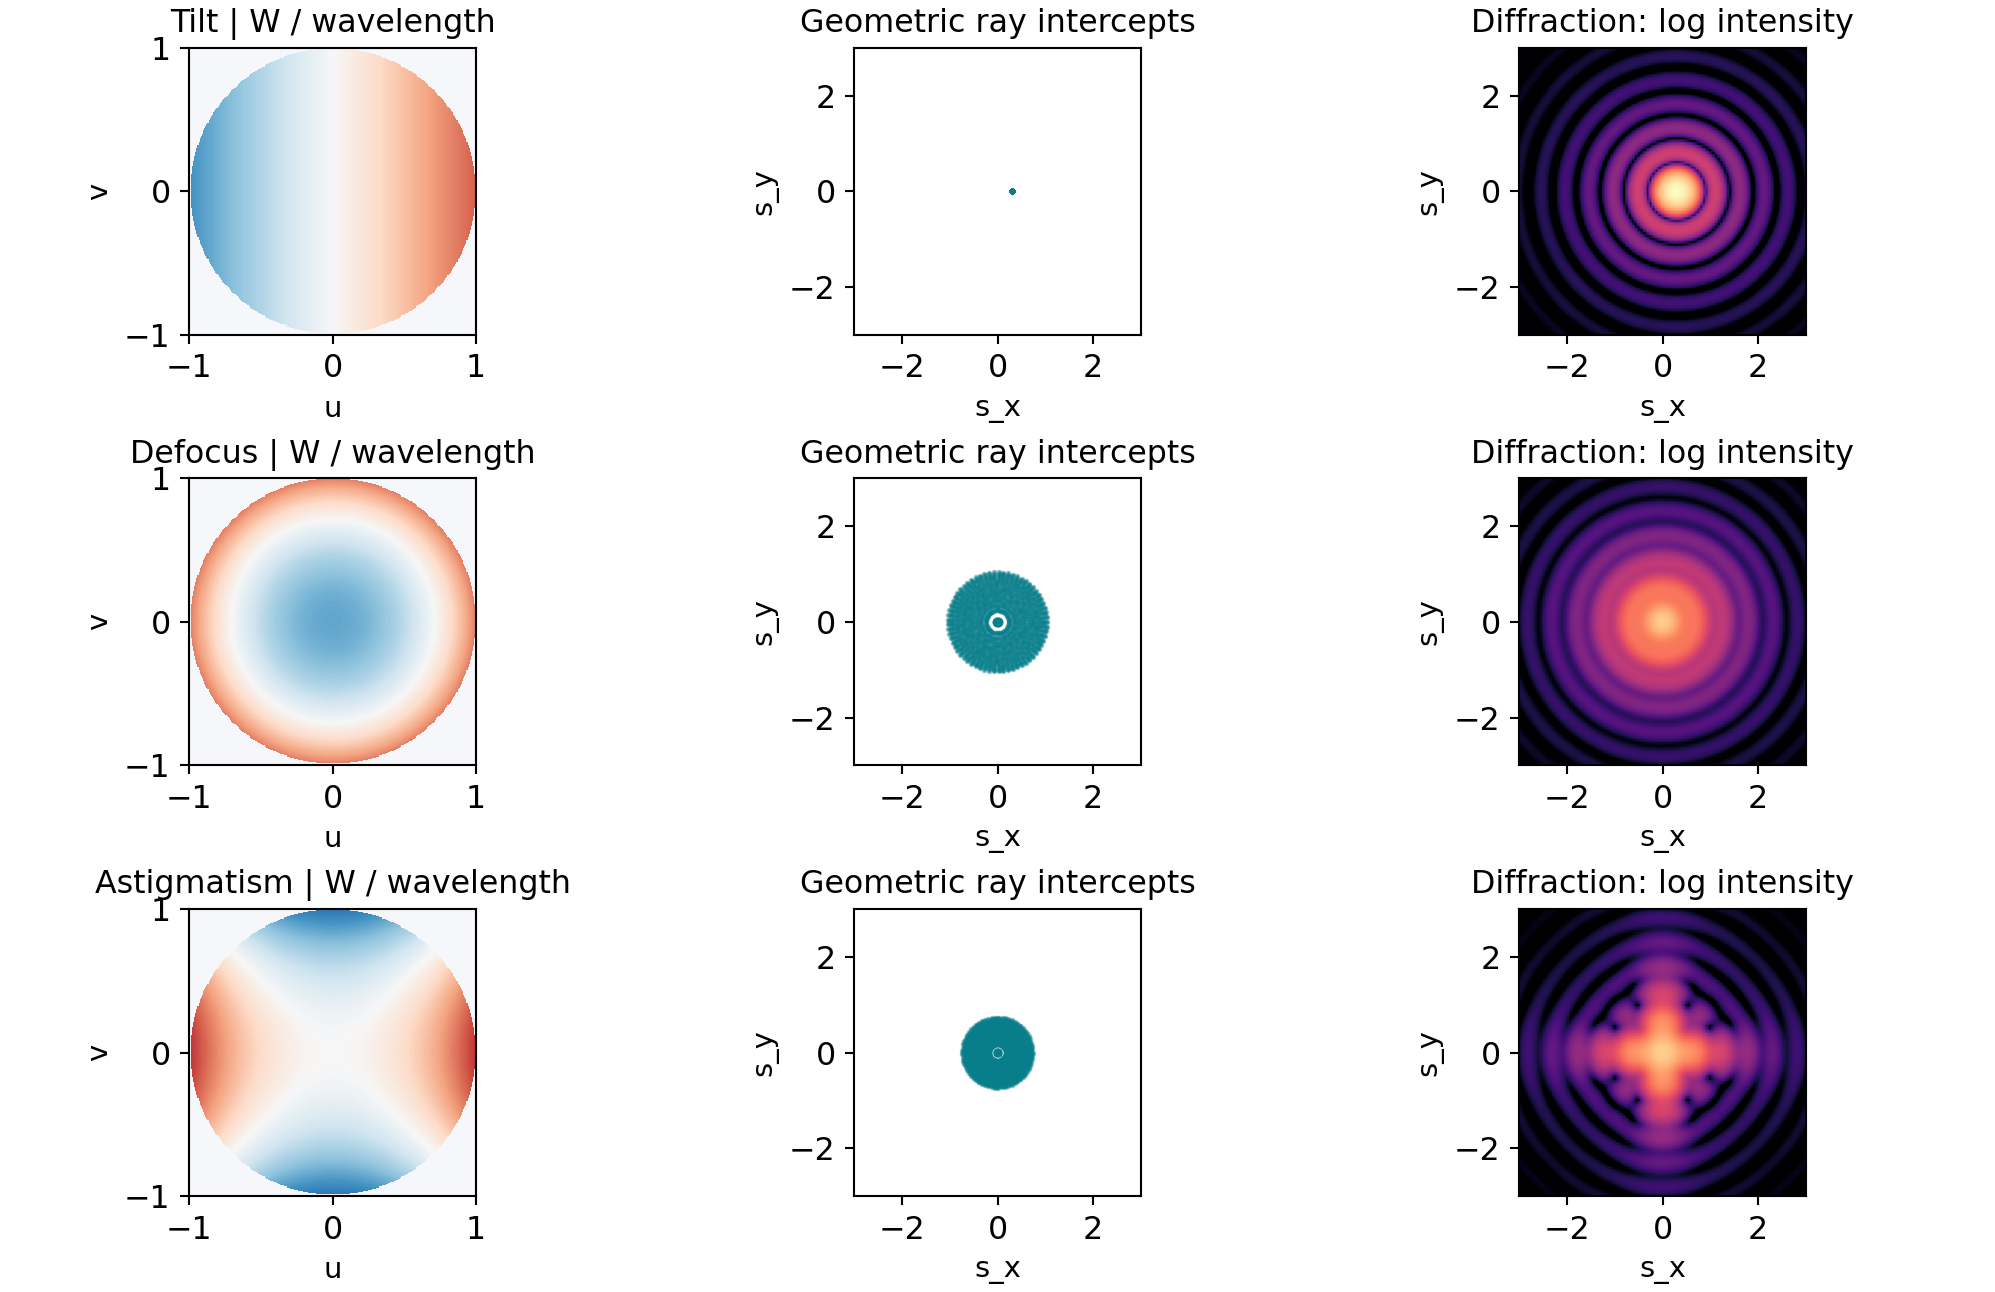
\includegraphics[width=.98\textwidth]{figures/pupil_ray_psf_1.png}
% \caption{Tilt, defocus, and astigmatism at the same coefficient $c/\lambda_0=0.15$. OPD colours share a $[-0.5,0.5]$-wave scale. Ray intercepts have no diffraction width. Intensities use a common logarithmic scale from $10^{-4}$ to one ideal peak. Image axes are $s_x=\NA\xi/\lambda_0$, $s_y=\NA\eta/\lambda_0$.}
% \label{fig:bridge}
% \end{figure}
% \begin{figure}[H]\centering
% 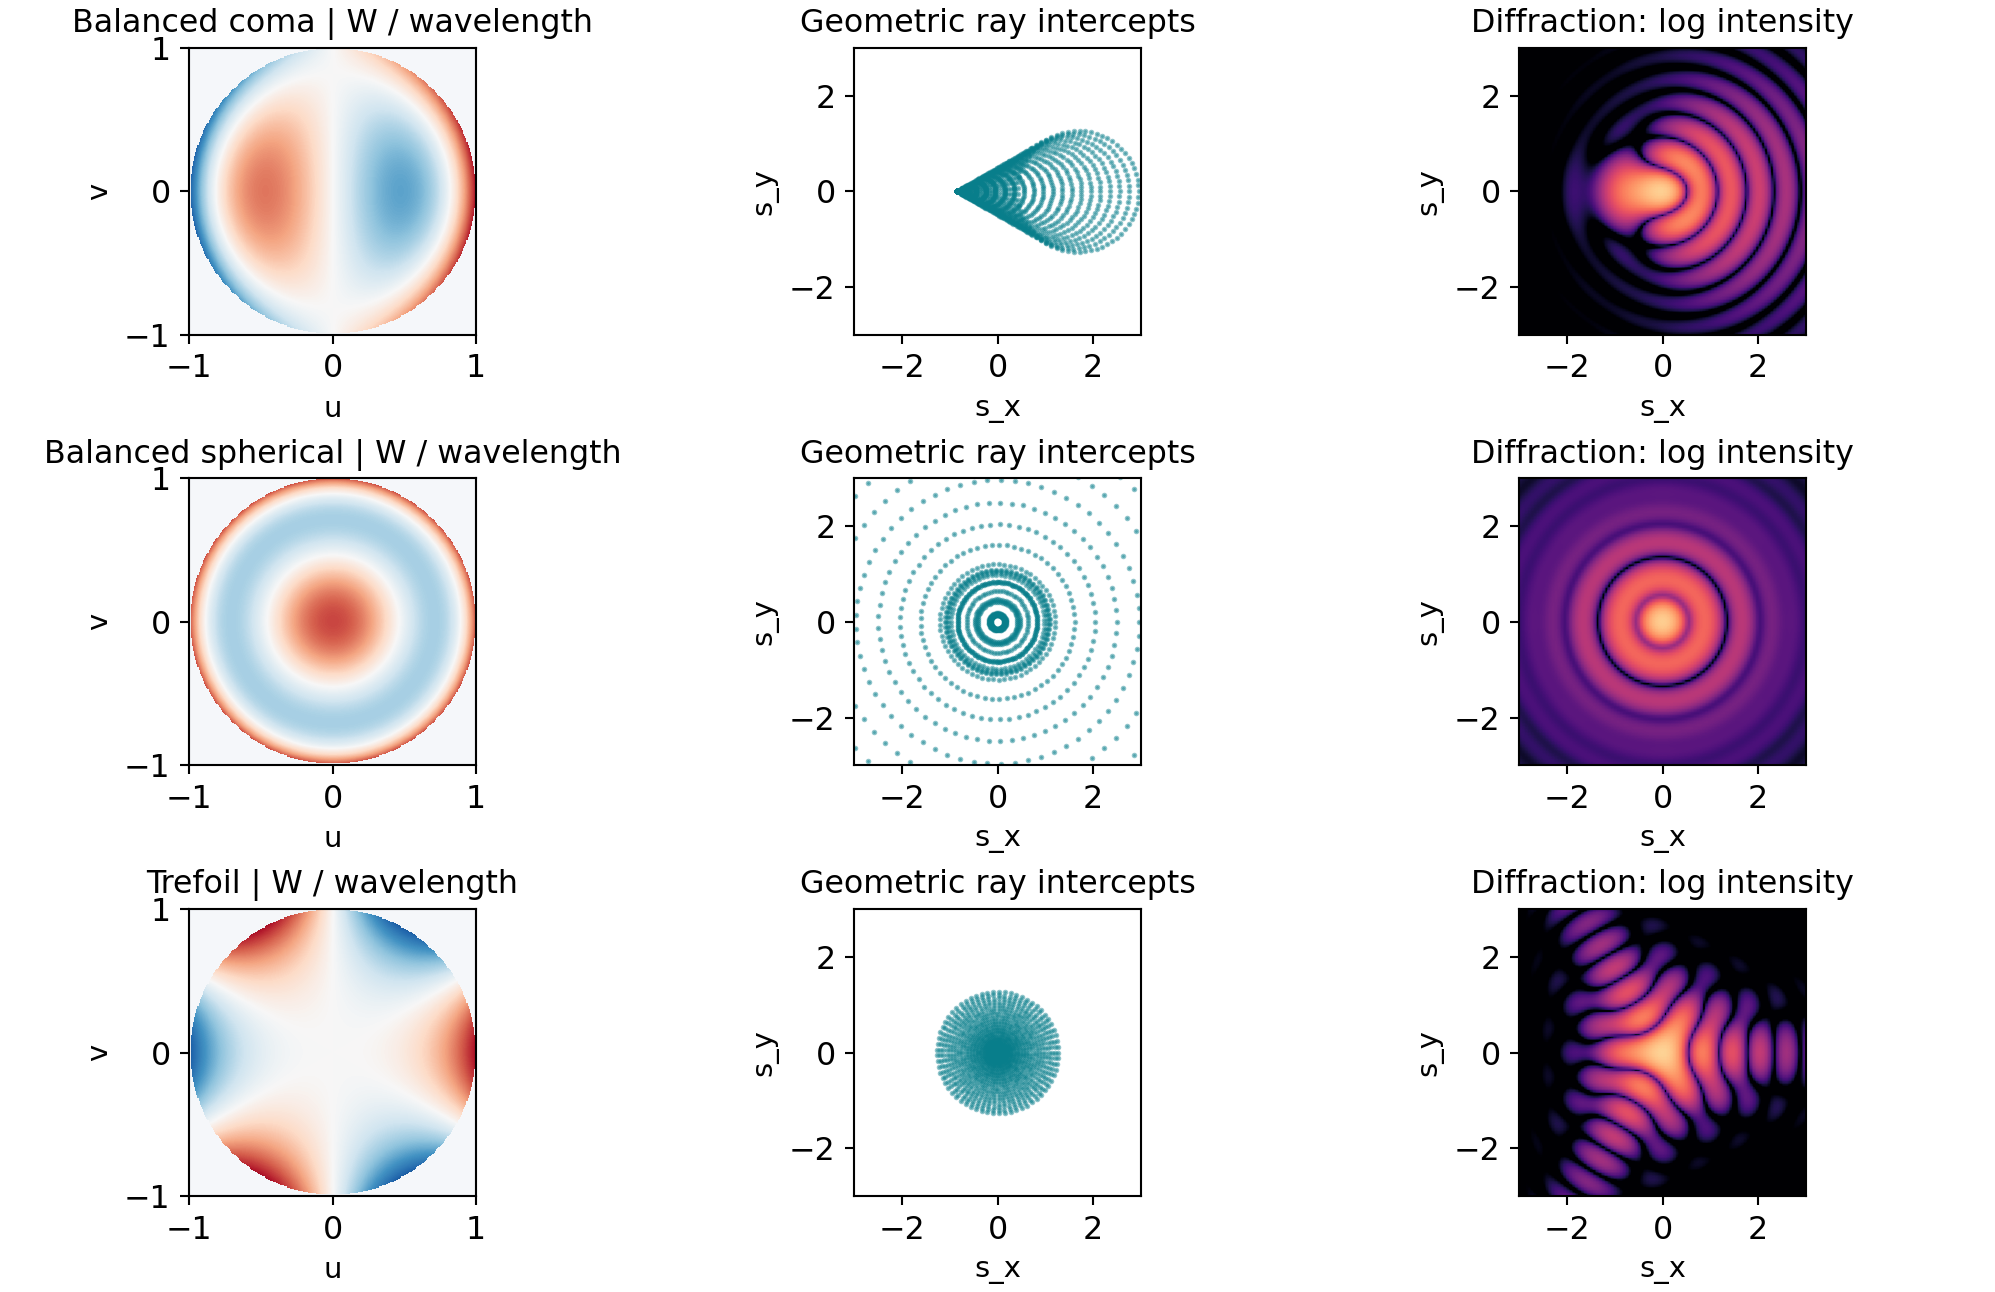
\includegraphics[width=.98\textwidth]{figures/pupil_ray_psf_2.png}
% \caption{Balanced coma, balanced spherical aberration, and trefoil, using exactly the same coefficient, OPD colour limits, image coordinates, and intensity normalization as Fig.~\ref{fig:bridge}. The lower-order balance changes the slopes; the diffraction law is unchanged.}
% \end{figure}

\section{Small-error RMS: useful, but not sufficient}
For a uniform disk pupil at the reference image point, normalize the field by its unaberrated value:
\begin{equation}
\frac{U(0)}{U_0(0)}=\avg{\ee^{\ii\phi}},\qquad
\phi=\frac{2\pi W}{\lambda_0},\qquad
\avg{g}=\frac1\pi\int_0^{2\pi}\int_0^1g\rho\dd\rho\dd\theta.
\end{equation}
Expanding the exponential and retaining intensity terms through second order,
\begin{align}
\avg{\ee^{\ii\phi}}&\simeq1+\ii\avg\phi-\tfrac12\avg{\phi^2},\\
S_{\rm ref}&=\left|\avg{\ee^{\ii\phi}}\right|^2
\simeq1-\avg{\phi^2}+\avg\phi^2
=\boxed{1-\left(\frac{2\pi\sigma_W}{\lambda_0}\right)^2}.
\end{align}
Here $\sigma_W^2=\avg{(W-\avg W)^2}$. The widely used exponential
$S\simeq\exp[-(2\pi\sigma_W/\lambda_0)^2]$ has the same leading term, but is not an exact formula for arbitrary deterministic aberration. At $\sigma_W=\lambda_0/50$, it gives $S\simeq0.9843$.

\textbf{Three distinct ambiguities.}
\begin{enumerate}
\item \textbf{RMS degeneracy.} Many coefficient vectors have the same sum of squares. Equal RMS does not specify mode, orientation, placement, or a pattern's phase differences. Tilt can preserve the peak while shifting it; coma and astigmatism redistribute intensity differently.
\item \textbf{Measurement invariance.} Piston gives exactly the same intensity. If images are recentered, pure tilt also disappears from the retained data. For a real centrosymmetric pupil and even $W$, $U_{-W}(\mathbf s)=U_W^*(-\mathbf s)$ and $U_W(-\mathbf s)=U_W(\mathbf s)$, so a single in-focus point intensity cannot distinguish $W$ from $-W$. Additional planes or references can supply missing information.
\item \textbf{Metric compression.} Different images or wavefronts may share the same few CD, placement, or process-window metrics. Orthogonal pupil coordinates do not guarantee a unique inverse map from these observables.
\end{enumerate}
Strehl normally compares consistent \emph{peak} intensities. The displayed expansion first evaluates a fixed reference point; specify whether tilt or focus has been optimized. With nonuniform amplitude $A$, the coherent field average is weighted by $A$, not automatically by intensity $A^2$. The clear-disk RMS formula cannot be transferred silently to an obscured or apodized pupil.

